
\section{Appendix A}
\label{sec:appendix-a}

\subsection{Git Internals}
\subsubsection{Dictionary}
\label{subsec:git-internals}
\begin{description}
  \item[Git] -- is a simple key-value data store and stores 3 main types of Objects: blob, tree, commit, and one additional: tag.
  \item[Blob] -- content of file w/o filename.
  \item[Tree] -- A single tree object contains one or more entries, each of which is the SHA-1 hash of a blob or subtree with its associated mode, type, and filename.
  For example, the most recent tree in a project may look something like this:\\
  \\
  \code{\$ git cat-file -p master\^\{tree\}}\\
  \code{100644 blob a906cb2a4a904a152e80877d4088654daad0c859      README}\\
  \code{100644 blob 8f94139338f9404f26296befa88755fc2598c289      Rakefile}\\
  \code{040000 tree 99f1a6d12cb4b6f19c8655fca46c3ecf317074e0      lib}
  \begin{figure}[H]
    \centering
    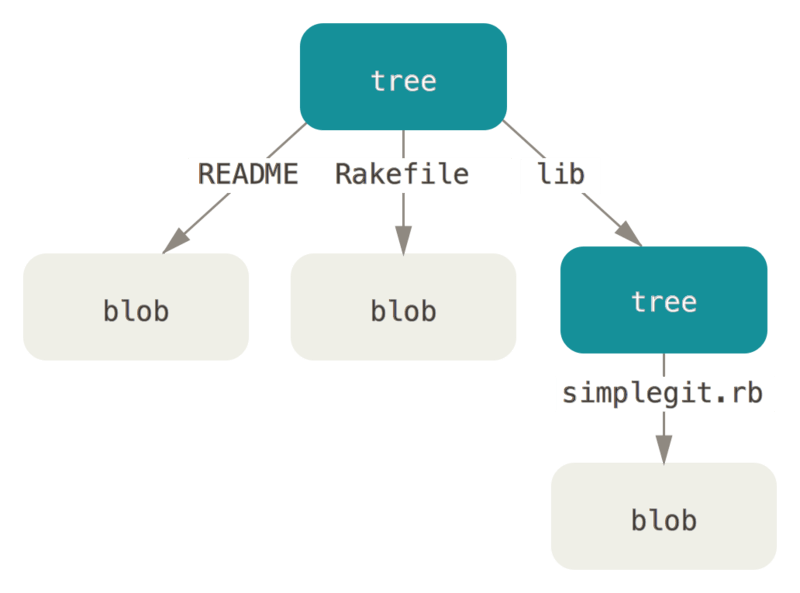
\includegraphics[width=\textwidth]{data-model-1.png}
    \label{fig:tree-objects}
  \end{figure}
  \item [Commit] is just a pointer to parent(previous) commit if any
  and to top-level tree for current one with some metadata
  (the author information and so on).
  \begin{figure}[H]
    \centering
    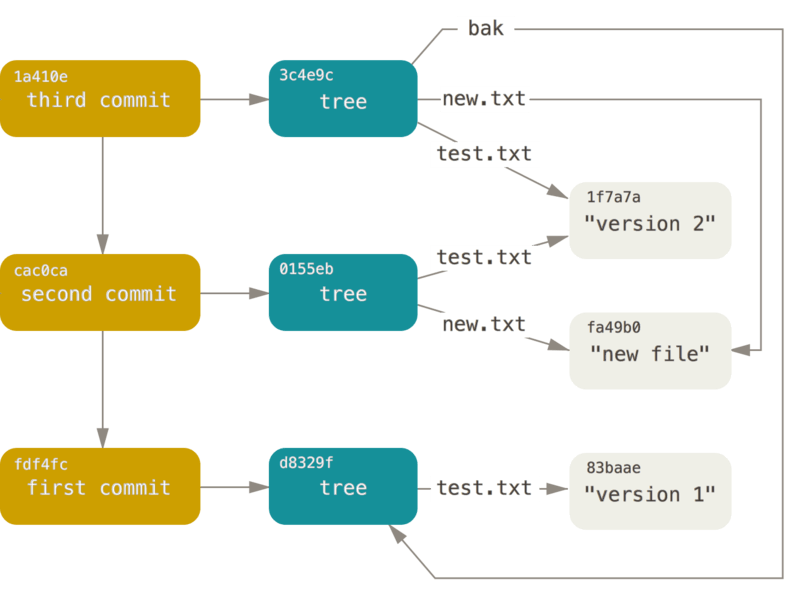
\includegraphics[width=\textwidth]{data-model-3.png}
    \label{fig:commit-objects}
  \end{figure}
\end{description}

{\large Other things, listed below, serve to make our interaction with these objects easier.
}
\begin{description}
  \item[Reference] - A file in which you could store SHA-1 value
  of a commit under a simple name, so you could use that simple name
  rather than the raw SHA-1 value.
  \item[Branch] is a simple pointer or reference to the head of a line of work(the latest commit) in .git/refs/heads.
  Branch name is mapped to the SHA of the commit that is latest for this branch.
  \begin{figure}[H]
    \centering
    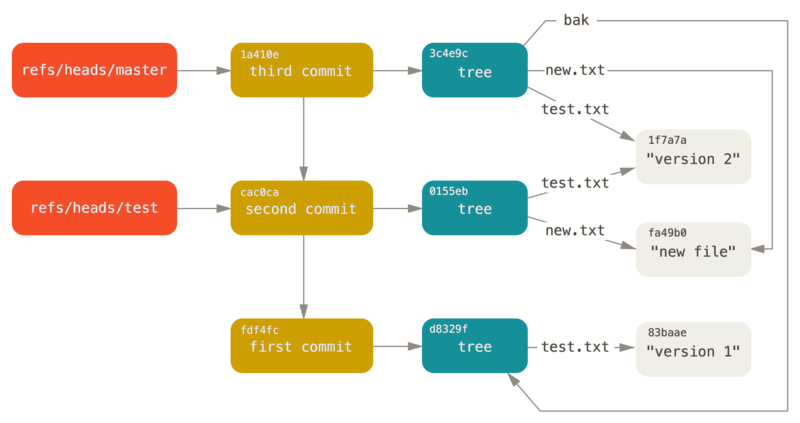
\includegraphics[width=\textwidth]{data-model-4.png}
    \label{fig:reference}
  \end{figure}
  When you run commands like \code{git branch <branch>},
  Git basically runs update-ref command to add the SHA-1
  of the last commit of the branch you're on into whatever
  new reference you want to create.
  So create branch is just create a reference to some commit.
  And delete branch is only delete reference.
  After branch deletion, all its objects will be available via their SHA.
  The same is for other reference under .git/refs
  \item[HEAD] Usually the HEAD file is a symbolic reference to the branch
  you're currently on.
  By symbolic reference, we mean that unlike a normal reference,
  it contains a pointer to another reference.\\
  If you look at the file, you'll normally see something like this:\\
  \\
  \code{\$ cat .git/HEAD}\\
  \code{ref: refs/heads/master}\\
  \\If you run \code{git checkout branch}, Git updates the file to look like this:\\
  \\
  \code{\$ cat .git/HEAD}\\
  \code{ref: refs/heads/test}\\

  When you run \code{git commit}, it creates the commit object,
  specifying the parent of that commit object to be whatever SHA-1 value
  the reference in HEAD points to.
  This commit also becomes a new head for a current branch.
  refs/heads/<branch-name> will be updated and map to the SHA
  of this new commit.
  When you do \code{git reset HEAD~1},
  it also only update refs/heads/<branch-name>.
  It takes SHA of parent commit of current head commit.
  \item[Tag (lightweight)] It's like a branch reference, but it never moves - it always points to the same commit but gives it a friendlier name.\\
  You can create, update and delete such a tag, and no objects would be affected.
  It's only a reference.
  \item[Tag (annotated)] - tag object, that points to commit or any other object amd contains metadata, and a reference to this tag object.

  Use \code{git push --follow-tags} if you want to push your annotated tag to remote repo.
  To delete a tag on your local repository, you can use \code{git tag -d <tagname>}.
  To delete a remote tag: \code{git push origin --delete <tagname>}.

  Both operation only delete a reference in .git/refs/tag.
  Tag object wouldn't be removed.
\end{description}

\subsubsection{Objects update workflow}
The most important updates of remote repo for us listed in the table below:

\begin{table}[H]
  \hskip-2.0cm\begin{tabular}{|l|l|l|}
                \hline
                action                                                               & git commands                                                                                                                                                                                                                                    & git server changes                                                                                                                                                                                                                                        \\ \hline
                create branch                                                        & \begin{tabular}[c]{@{}l@{}}git push  \textless{}remote-name\textgreater \\  \textless{}branch-name\textgreater{}:\textless{}remote-branch-name\textgreater{}\end{tabular}                                                                       & \begin{tabular}[c]{@{}l@{}}A new reference \\ .git/refs/heads/\textless{}branch-name\textgreater \\ will be created.\end{tabular}                                                                                                                         \\ \hline
                delete branch                                                        & \begin{tabular}[c]{@{}l@{}}git push  \textless{}remote-name\textgreater \\ :\textless{}remote-branch-name\textgreater\\ OR\\ git push \textless{}remote-name\textgreater  \\ --delete  \textless{}remote-branch-name\textgreater{}\end{tabular} & \begin{tabular}[c]{@{}l@{}}The existing reference \\ .git/refs/heads/\textless{}branch-name\textgreater \\ will be removed.\end{tabular}                                                                                                                  \\ \hline
                create tag                                                           & \begin{tabular}[c]{@{}l@{}}git push \textless{}remote-name\textgreater \\ \textless{}tag-name\textgreater{}:\textless{}remote-tag-name\textgreater{}\end{tabular}                                                                               & \begin{tabular}[c]{@{}l@{}}A new reference \\ .git/refs/tags/\textless{}tag-name\textgreater \\ will be created.\\ For annotated tags only:\\ new tag-object also will be created\\ .git/objects/SHA{[}0,2{]}/SHA{[}2,40{]}\end{tabular}                  \\ \hline
                delete tag                                                           & git push \textless{}remote-name\textgreater :\textless{}tag-name\textgreater{}                                                                                                                                                                  & \begin{tabular}[c]{@{}l@{}}The existing reference \\ .git/refs/tags/\textless{}tag-name\textgreater\\  will be removed.\\ For annotated tags:\\ tag-object won't be removed or updated\\ For lightweight tags:\\ tag-object doesn't exist\end{tabular}    \\ \hline
                \begin{tabular}[c]{@{}l@{}}create ref\\ delete ref\end{tabular}      &                                                                                                                                                                                                                                                 & \begin{tabular}[c]{@{}l@{}}Reference is fully equal to branch,\\  it's just an alias.\end{tabular}                                                                                                                                                        \\ \hline
                \begin{tabular}[c]{@{}l@{}}update branch\\ (new commit)\end{tabular} & git push                                                                                                                                                                                                                                        & \begin{tabular}[c]{@{}l@{}}New objects will be created \\ (commit, tree, etc.).\\ The existing reference \\ .git/refs/heads/\textless{}remote-branch-name\textgreater \\ will be updated.\\ It will start pointing \\ to to this new commit.\end{tabular} \\ \hline
  \end{tabular}\label{tab:update-workflow}
\end{table}

\subsubsection{Git file storage internals}

\textbullet\textbf{\large{ loose object storage}}\\

As we metioned, a git repository take cares of several types of objects:
\code{blob}, \code{tree}, \code{commit}, \code{tag}. Let's take a look at the details of object storage:\\

git default write the objects to directory \code{GIT\_DIR\footnote{the .git directory}/objects}.
Each object is named by a sha1 value for example \emph{\code{b98191cf971f2418e42877410a6c40fc112a0a93}}\\
it's storage path will be
\begin{center}
\emph{\code{GIT\_DIR/objects/b9/8191cf971f2418e42877410a6c40fc112a0a93}}
\end{center}
the directories under \code{GIT\_DIR/objects} is named by \code{SHA[0,2]} of objects' sha1 value,
this can avoid too much files in one directory because some filesystem has the max link number of files,
such as ext3 has the definition:
\begin{flushleft}
  \code{include/linux/ext3\_fs.h:\#define EXT3\_LINK\_MAX           32000}
\end{flushleft}

One object file is consist of three portions:
\begin{description}
  \item[type] can be one of `blob', `tree', `commit', `tag'
  \item[size] the number of bytes of the content
  \item[content] the content of object
\end{description}

and the object file will be compressed using zlib:

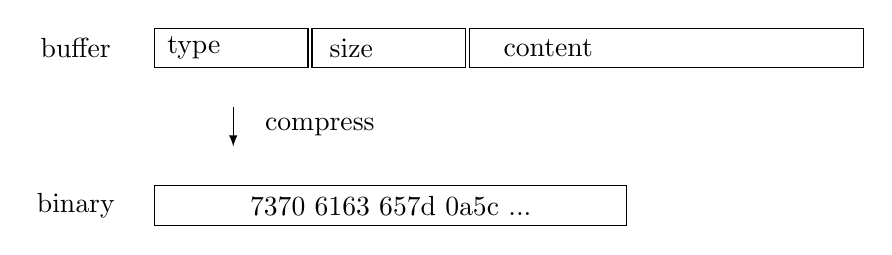
\begin{tikzpicture}
  \node at (0,0.25) {binary};
  \node at (4,0.25) {\code{7370 6163 657d 0a5c ...}};
  \draw (1,0) rectangle (7,0.5);
  \node at (3.1,1.25) {compress};
  \draw[-latex] (2,1.5) -- (2,1);
  \node at (0,2.25) {buffer};
  \node at (1.5,2.25) {type};
  \node at (3.5,2.25) {size};
  \node at (6,2.25) {content};
  \draw (1,2) rectangle (2.95,2.5);
  \draw (3,2) rectangle (4.95,2.5);
  \draw (5,2) rectangle (10,2.5);
\end{tikzpicture}

the compression level can be set by `\textbf{\code{core.compression}}' or `\textbf{\code{core.loosecompression}}'.
\\

\textbullet\textbf{\large{ pack file storage}}\\

When we do \emph{\code{git gc}} or \emph{\code{git repack}}, pack files with the suffix \code{.pack}
maybe be created under directory \emph{\code{GIT\_DIR/objects/pack}}. A pack is a collection of objects,
individually compressed, with delta compression applied, stored in a single file, with an associated
index file. Packs are used to reduce the load on mirror systems, backup engines, disk storage, etc.

\begin{lstlisting}[basicstyle=\ttfamily]
$ tree .git/objects/pack
.git/objects/pack
|-- pack-24fcb83682e5a2848ef7bd00a9eda0bff1a372fc.idx
|-- pack-24fcb83682e5a2848ef7bd00a9eda0bff1a372fc.pack
|-- pack-915d8b4ae03b03179912c589cee932e5a990b7f0.idx
|-- pack-915d8b4ae03b03179912c589cee932e5a990b7f0.pack
|-- ...
\end{lstlisting}

Conceptually there are only four object types in a pack file: commit, tree, tag and blob.
However to save space, an object could be stored as a ``delta'' of another ``base'' object.
These representations are assigned new types \code{ofs-delta} and \code{ref-delta}.

\begin{description}
  \item[delta object]
    Both ofs-delta and ref-delta store the ``delta'' to be applied to another object
    (called `base object') to reconstruct the object. The difference between them is,
    ref-delta directly encodes 20-byte base object name. If the base object is in the same pack,
    ofs-delta encodes the offset of the base object in the pack instead.
  \item[base object]
    The base object could also be deltified if it's in the same pack.
    Ref-delta can also refer to an object outside the pack. When stored on disk however,
    the pack should be self contained to avoid cyclic dependency.
\end{description}

And usualy we have lots of versions of a single file in a repository, a new pack file will
store the last version's content as the base object, and computes the earlier versioins to
to be delta objects and store them referring to the base object:

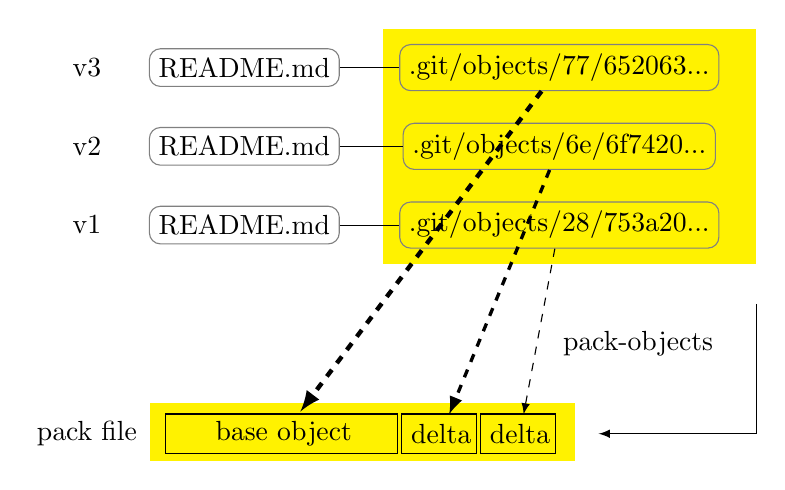
\begin{tikzpicture}
  % loose objects
  \filldraw[fill=yellow, draw=white] (3.75,2.5) rectangle (8.5,5.5);

  \node at(0,5){v3};
  \node[rectangle,rounded corners, draw=gray,] (v3) at(2,5){README.md};
  \node[rectangle,rounded corners, draw=gray,] (v3obj) at(6,5){.git/objects/77/652063...};
  \node at(0,4){v2};
  \node[rectangle,rounded corners, draw=gray,] (v2) at(2,4){README.md};
  \node[rectangle,rounded corners, draw=gray,] (v2obj) at(6,4){.git/objects/6e/6f7420...};
  \node at(0,3){v1};
  \node[rectangle,rounded corners, draw=gray,] (v1) at(2,3){README.md};
  \node[rectangle,rounded corners, draw=gray,] (v1obj) at(6,3){.git/objects/28/753a20...};
  \draw (v3) -- (v3obj);
  \draw (v2) -- (v2obj);
  \draw (v1) -- (v1obj);

  % arrow
  \draw (8.5,2) -- (8.5,0.35);
  \draw[-latex] (8.5,0.35) -- (6.5,0.35);
  \node at(7,1.5){pack-objects};

  % pack file
  \filldraw[fill=yellow, draw=white] (0.8,0) rectangle (6.2,0.75);
  \node at (0,0.35) {pack file};
  \node (base) at (2.5,0.35) {base object};
  \node (deltav2) at (4.5,0.35) {delta};
  \node (deltav1) at (5.5,0.35) {delta};
  \draw (1,0.1) rectangle (3.95,0.6);
  \draw (4,0.1) rectangle (4.95,0.6);
  \draw (5,0.1) rectangle (5.95,0.6);

  \draw[dashed, ultra thick, -latex] (v3obj) -- (base);
  \draw[dashed, very thick, -latex] (v2obj) -- (deltav2);
  \draw[dashed, -latex] (v1obj) -- (deltav1);
\end{tikzpicture}

Usually objects contained in the pack are compressed using zlib, the compression level
can be set by `\textbf{\code{core.compression}}' or `\textbf{\code{pack.compression}}'.

When objects contained in the pack are stored using delta compression. The objects
are first internally sorted by type, size and optionally names and compared against
the other objects to see if using delta compression saves space. `\textbf{\code{pack.depth}}'
limits the maximum delta depth; Making it too deep affects the performance on the unpacker side,
because delta data needs to be applied that many times to get to the necessary object.
\\

To quickly find objects in the pack file, an associated index file is created with the
\emph{\href{https://github.com/git/git/blob/master/Documentation/technical/pack-format.txt\#L161}{format}},
And `\emph{\code{git index-pack}}' can be used to regenerate the *.idx file on the *.pack file.
\\

\textbullet\textbf{\large{ when pack file is created}}\\

When we talk about the pack files, we said that packs are used to reduce the load on mirror systems,
backup engines, disk storage, etc. So pack files will created in several scenes:

\begin{description}
  \item[git gc] `\emph{\code{git gc}}' runs a number of housekeeping tasks within the repository,
    such as compressing file revisions (to reduce disk space and increase performance), removing
    unreachable objects which may have been created from prior git commands.
    We can run it manually, and it may create a new pack file.
  \item[git repack] `\emph{\code{git repack}}' is used to combine all objects that do not currently
    reside in a pack file into a pack. It can also be used to re-organize existing packs into
    a single, more efficient pack.
  \item[git push] `\emph{\code{git push}}' will run \code{send-pack} to connects to the remote side,
    it gets one file descriptor which is either a socket (over the network) or a pipe (local).
    What's written to this file descriptor goes to `\emph{\code{git-receive-pack}}' to be unpacked.
    We can get the following pipeline flow from\\
    \emph{\href{https://github.com/git/git/blob/master/Documentation/technical/send-pack-pipeline.txt}{Documentation/technical/send-pack-pipeline.txt}}:
    \begin{lstlisting}[basicstyle=\ttfamily]
    send-pack
       |
       pack_objects() --> fd --> receive-pack
          | ^ (pipe)
          v |
       (child)
    \end{lstlisting}
    so we can see that `\emph{\code{git push}}' will create a pack file and send it to the remote side.
  \item[git-receive-pack] As menthioned above, `\emph{\code{git-receive-pack}}' will receive a pack file
    from `\emph{\code{git push}}'. And `\emph{\code{git receive-pack}}' will also forked a child
    `\emph{\code{git gc --auto --quiet}}' to check if there are too many loose objects to pack.
    Ususaly the threshold is 6700 loose files, we can set it by `\textbf{\code{gc.auto}}'.
  \item[git-upload-pack] When clients runs `\emph{\code{git clone}}' or `\emph{\code{git fetch}}', the
    client connects to the remote side and invokes `\emph{\code{git-upload-pack}}'.
    `\emph{\code{git-upload-pack}}' will communicate with client and compute how many objects the client
    want then fork and exec child `\emph{\code{git-pack-objects}}' to create a pack file for all the
    needed objects and pipe the pack file to client.
    \begin{lstlisting}[basicstyle=\ttfamily]
    upload-pack
       |
       pack_objects() --> fd --> fetch-pack
          | ^ (pipe)
          v |
       (child)
    \end{lstlisting}

    We can also use the `\textbf{\code{repack.writeBitmaps}}' to let git write a bitmap index when packing
    all objects to disk (e.g., when git repack -a is run). This index can speed up the "counting
    objects" phase of subsequent packs created for clones and fetches, at the cost of some disk space
    and extra time spent on the initial repack.

\end{description}
